\documentclass[12pt,a4paper]{article}
\usepackage[T1]{fontenc}
\usepackage{amsmath}
\usepackage{amssymb}
\usepackage{graphicx}
\usepackage[UTF8,heading=true]{ctex}
\usepackage{geometry}
\usepackage{diagbox}
\usepackage[]{float}
\usepackage{xeCJK}
\usepackage{indentfirst}
\usepackage{multirow}
\usepackage[section]{placeins}
\usepackage{caption}
\usepackage{listings}
\usepackage{xcolor}

% 设置代码块样式
\lstset{
  frame=tb,
  aboveskip=3mm,
  belowskip=3mm,
  showstringspaces=false,
  columns=flexible,
  framerule=1pt,
  rulecolor=\color{gray!35},
  backgroundcolor=\color{gray!5},
  basicstyle={\small\ttfamily},
  numbers=none,
  numberstyle=\tiny\color{gray},
  keywordstyle=\color{blue},
  commentstyle=\color{green!50!black},
  stringstyle=\color{mauve},
  breaklines=true,
  breakatwhitespace=true,
  tabsize=3,
}

\setCJKfamilyfont{zhsong}[AutoFakeBold = {5.6}]{STSong}
\newcommand*{\song}{\CJKfamily{zhsong}}

\geometry{a4paper,left=2cm,right=2cm,top=0.75cm,bottom=2.54cm}

\newcommand{\experiName}{prj4}%实验名称
\newcommand{\name}{28}
\newcommand{\student}{刘景平、张钰堃、付博宇}%姓名
\newcommand{\others}{$\square$}
\newcommand{\sectionfont}{\song\textbf}

\ctexset{
    section={
        format+=\raggedright
    },
    subsection={
        name={\quad,.}
    },
    subsubsection={
        name={\qquad,.}
    }
}

\begin{document}
\noindent

\begin{center}

    \textbf{\song \zihao{-2} \ziju{0.5} 计算机体系结构(研讨课)实验报告}
    
\end{center}


\begin{center}
    \kaishu \zihao{5}
    \noindent \emph{实验项目}\underline{\makebox[5em][c]{\experiName}}
    \emph{小组编号}\underline{\makebox[5em][c]{\name}} 
    \emph{组员姓名}\underline{\makebox[20em][c]{\student}}
    {\noindent}
    \rule[5pt]{17.7cm}{0.2em}

\end{center}


\section{\sectionfont 逻辑电路结构与仿真波形的截图及说明}
    \subsection{exp12}
        \subsubsection{增加CSR模块}
            1.需要为CSR模块单独写一个verilog文件,作为专用于CSR的寄存器堆,按照教材上的指导加入一系列输入输出信号,
            并在头文件中加入每个CSR的寄存器号,每个CSR各部分的位置等信息:
            \begin{figure}[H]
                \centering
                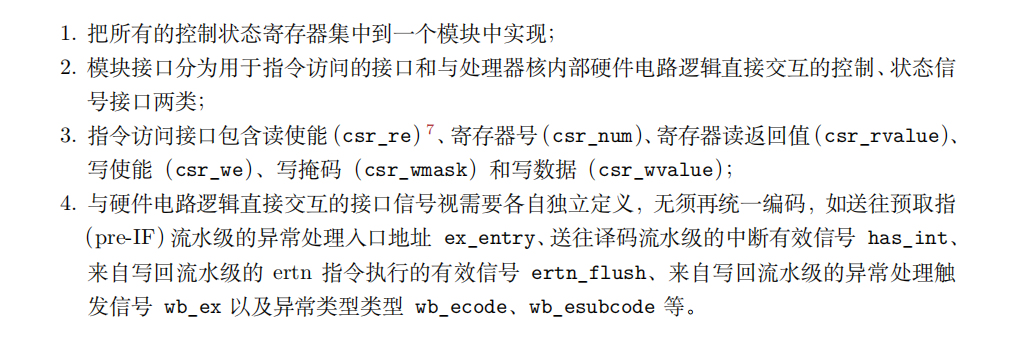
\includegraphics[width=0.8\textwidth]{创建CSR-1.png}
                \caption{讲义上关于创建CSR模块的指导}
            \end{figure}

            \begin{figure}[H]
                \centering
                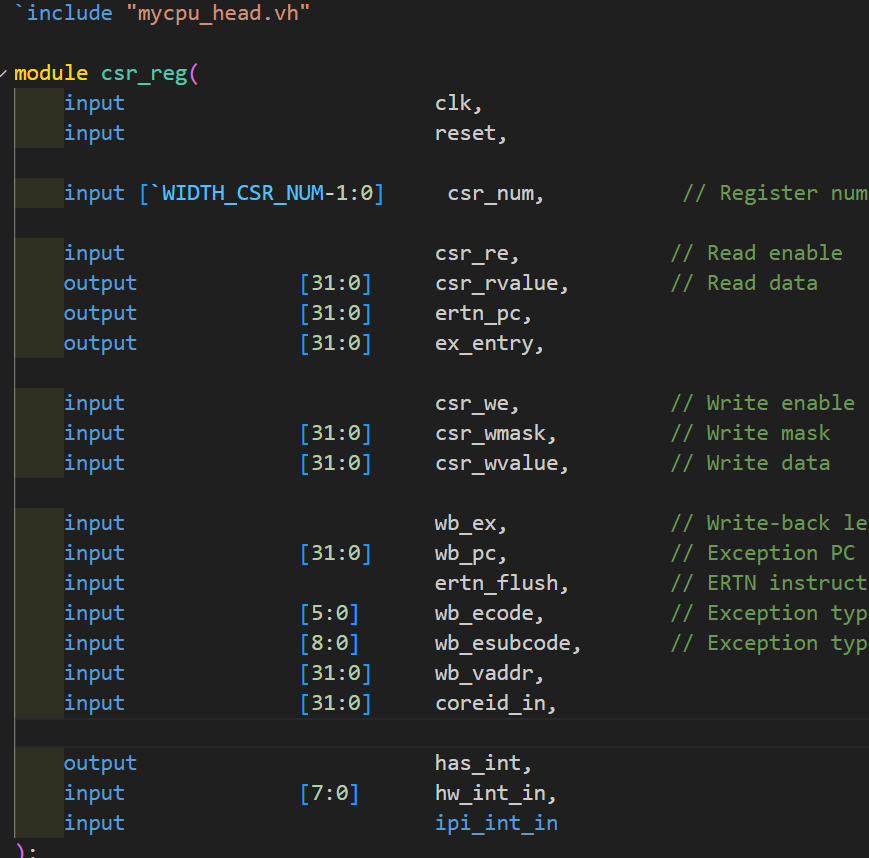
\includegraphics[width=0.8\textwidth,height=0.4\textheight]{修改头文件.png}
                \caption{创建CSR模块}
            \end{figure}

            \begin{figure}[H]
                \centering
                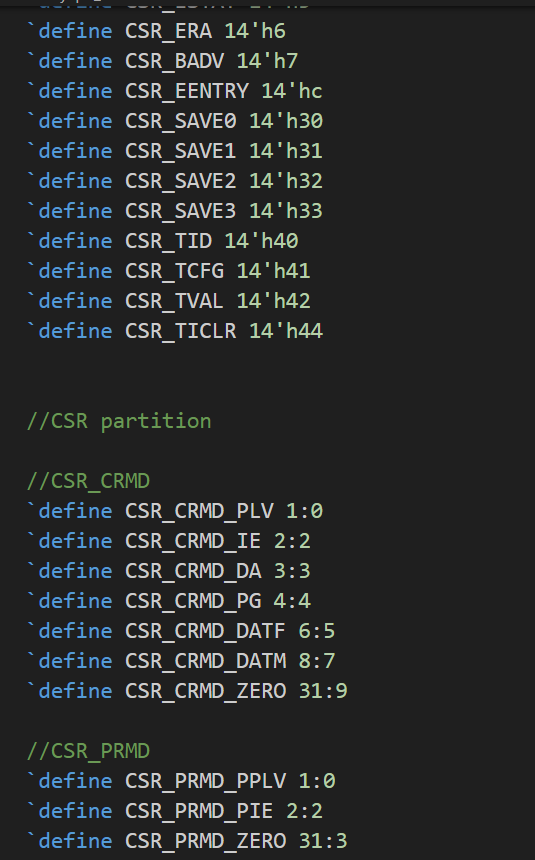
\includegraphics[width=0.8\textwidth,height=0.5\textheight]{创建CSR-2.png}
                \caption{修改头文件}
            \end{figure}
            \par
            2.根据讲义上的例子添加CRMD、PRMD、ESTAT、ERA、EENTRY、SAVE0~3八个控制状态寄存器。并按照指令集手册的要求添加关于read value的设置
            \begin{figure}[H]
                \centering
                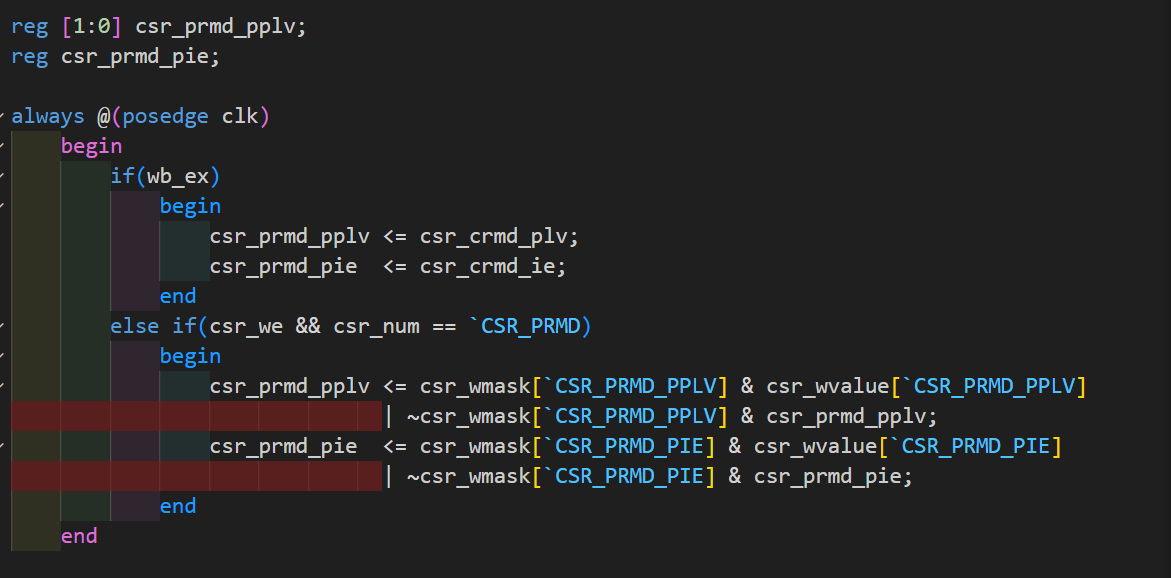
\includegraphics[width=0.8\textwidth]{PRMD.png}
                \caption{PRMD寄存器的设置}
            \end{figure}

            \begin{figure}[H]
                \centering
                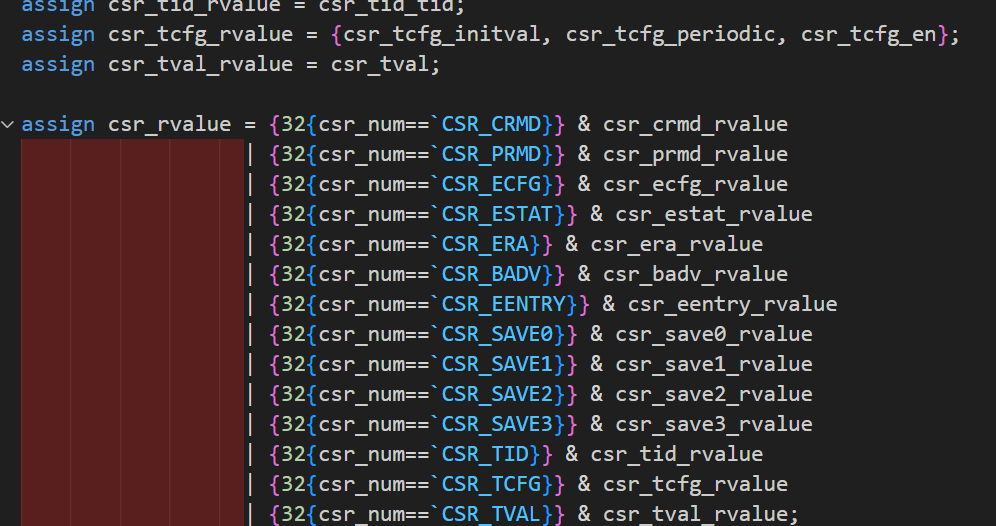
\includegraphics[width=0.8\textwidth]{rvalue.png}
                \caption{设置rvalue}
            \end{figure}
            \par
        
        \subsubsection{修改五个流水线模块}
            1.在IF中对nextpc进行修改,加入出现中断和例外,以及异常处理返回的情况
            \begin{lstlisting}[language=Verilog]
                wire [31:0] next_pc;    //nextpc from branch or sequence
                assign next_pc = (has_int || wb_ex)? ex_entry : ertn_flush? ertn_pc : br_taken? br_target : seq_pc;
            \end{lstlisting}
            \par
            2.在ID模块中加入对CSR读写指令有关的译码信号并增加和CSR有关的阻塞;
            \begin{lstlisting}[language=Verilog]
                wire csr_crush;
                assign csr_crush = (es_csr && (ex_crush1 || ex_crush2)) || (ms_csr && (mem_crush1 || mem_crush2)); 
            \end{lstlisting}

            \begin{figure}[H]
                \centering
                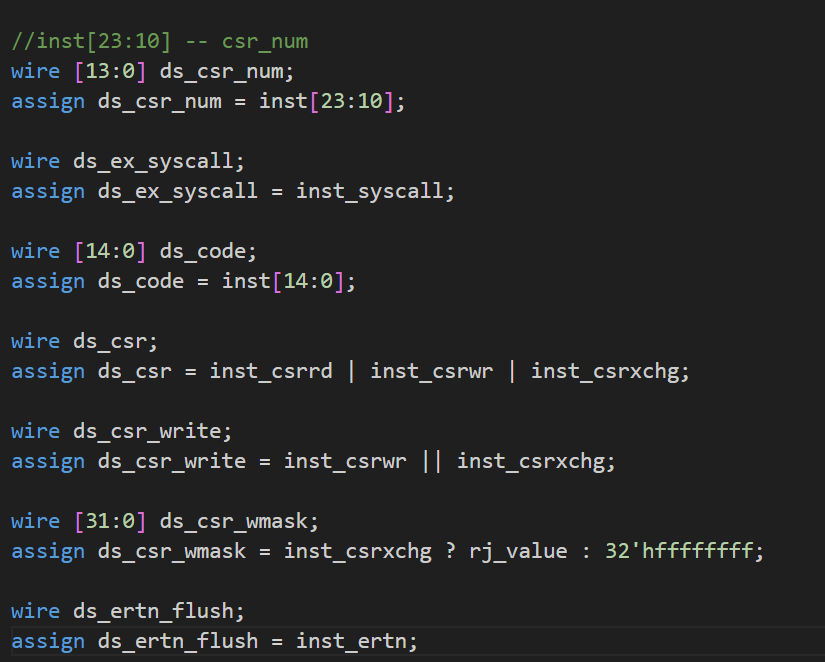
\includegraphics[width=0.8\textwidth,height=0.3\textheight]{csr读写译码.png}
                \caption{csr读写译码}
            \end{figure}
            \par
            3.在遇到ertn指令或者遇到中断和例外时,需要情况流水级间缓存:
            \begin{figure}[H]
                \centering
                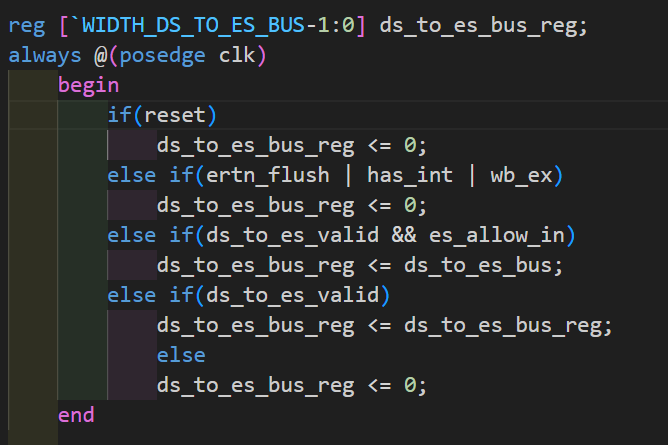
\includegraphics[width=0.8\textwidth]{清空流水级缓存.png}
                \caption{清空流水级间缓存}
            \end{figure}
            \par
            4.在最后一级WB级进行中断与异常的判断:
            \begin{figure}[H]
                \centering
                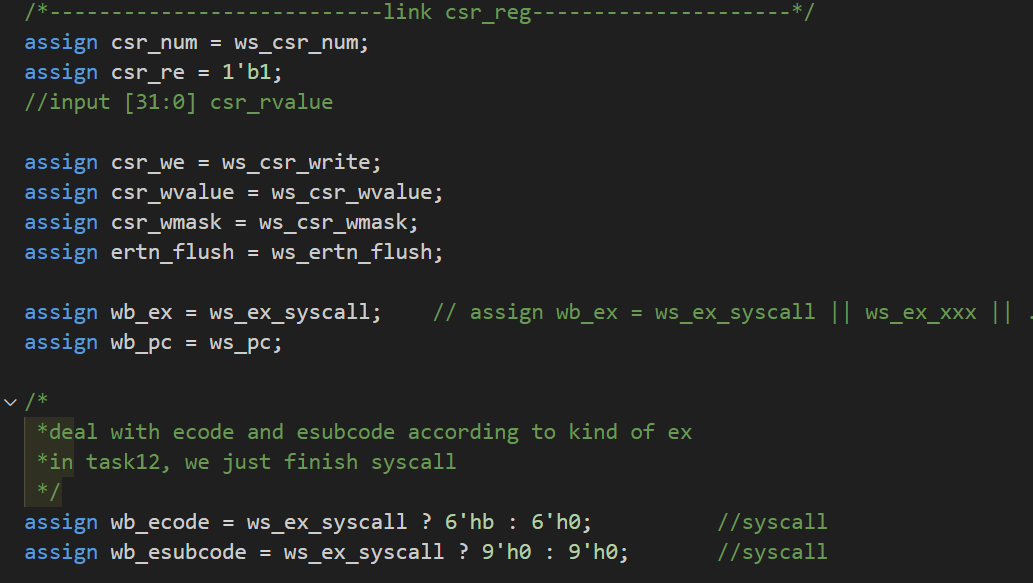
\includegraphics[width=0.8\textwidth]{在最后一级判断中断与异常.png}
                \caption{在最后一级判断中断与异常}
            \end{figure}
                
        
            
    \subsection{exp13}
        \subsubsection{添加异常、中断支持}
          1.根据讲义提供的思路,添加本次实验所要求的中断及异常的判定信号,以及对应的判定逻辑。
          \par
          \begin{lstlisting}[language=Verilog]
          assign fs_exc_ADEF = inst_sram_en && (fetch_pc[1] | fetch_pc[0]);
    
          assign      ds_exc_INE = ~(inst_add_w | inst_sub_w | inst_slt | inst_sltu 
            | inst_nor | inst_and | inst_or | inst_xor | inst_slli_w 
            | inst_srli_w | inst_srai_w | inst_addi_w | inst_ld_w | inst_st_w 
            | inst_jirl | inst_b | inst_bl | inst_beq | inst_bne | inst_lu12i_w 
            | inst_slti | inst_sltiu | inst_andi | inst_ori | inst_xori | inst_sll_w 
            | inst_srl_w | inst_sra_w | inst_pcaddu12i | inst_mul_w | inst_mulh_w 
            | inst_mulh_wu | inst_div_w | inst_div_wu | inst_mod_w | inst_mod_wu 
            | inst_blt | inst_bge | inst_bltu | inst_bgeu | inst_st_b | inst_st_h 
            | inst_ld_b | inst_ld_h | inst_ld_bu | inst_ld_hu
            | inst_csrrd | inst_csrwr | inst_csrxchg | inst_ertn | inst_syscall
            | inst_rdcntvl_w | inst_rdcntvh_w | inst_rdcntid | inst_break) && (ds_pc != 32'b0) ;


          //exp13 ALE exception
            wire ld_st_w,ld_st_h;
            assign ld_st_w = es_st_op[0] | (es_ld_op[1:0] == 2'b0 & es_res_from_mem);
            assign ld_st_h = es_st_op[2] | es_ld_op[1];
            assign es_exc_ALE = ((ld_st_w & (es_unaligned_addr != 2'b0)) | (ld_st_h & (es_unaligned_addr[0]))) & es_valid;
            //exp13 int
            assign has_int = ((csr_estat_is[11:0] & csr_ecfg_lie[12:0]) != 12'b0)
                && (csr_crmd_ie == 1'b1);
            
          \end{lstlisting}
          根据讲义内容,异常相当于给异常流水线打上对应标签,因此需要将异常标签通过流水级间总线进行传递,这里以EXE级向MEM级传递为例
          
            \begin{lstlisting}[language=Verilog]
            //exp13
            assign es_to_ms_bus[173:173] = es_exc_ADEF;
            assign es_to_ms_bus[174:174] = es_exc_INE;
            assign es_to_ms_bus[175:175] = es_exc_ALE;
            assign es_to_ms_bus[176:176] = es_exc_break;
            assign es_to_ms_bus[177:177] = es_has_int;
            assign es_to_ms_bus[209:178] = es_vaddr;
          \end{lstlisting}
          2.为了做到精确异常,需要实现异常时清空流水线,异常流水级后不能产生任何运行效果.这里重点关注紧跟在异常流水级之后的st类指令。
          \begin{lstlisting}[language=Verilog]
          //EX.v
            wire if_es_has_int;
            assign if_es_has_int = es_ex_syscall || es_ertn_flush || es_exc_ADEF || es_exc_ALE || es_exc_INE || es_exc_break || es_has_int || wb_ex;
            
            assign data_sram_en    = 1'b1;   
            assign data_sram_wen   = (es_mem_we && es_valid && ~has_int && ~if_ms_has_int && ~wb_ex && ~if_es_has_int & ~ertn_flush & ~es_ertn_flush) ? w_strb : 4'b0000;
            assign data_sram_addr  = (es_mul_op != 0) ? {es_mul_result[31:2],2'b00} : {es_alu_result[31:2],2'b00};
            assign data_sram_wdata = real_wdata;        
            
          \end{lstlisting}
        
        \subsubsection{增加控制状态寄存器}
        讲义针对如何添加ECFG,BADV,TID,TCFG,TVAL,TICLR控制状态寄存器以及如何维护不同寄存器的各个域均有详细描述,按照小组之前的代码框架对讲义上的实现方法进行微调,与exp12整体框架相同,具体代码也在书中多有提及,不再详细罗列。

        \subsubsection{增加计时器相关指令}
        添加rdcntvl.w,rdcntvh.w,rdcntid指令
        \par
        1.添加上述指令相关的译码信号。
        \begin{lstlisting}[language=Verilog]
        assign inst_rdcntid  =  op_31_26_d[6'h0] & op_25_22_d[4'h0] & op_21_20_d[2'h0] & op_19_15_d[5'h0] & (rk == 5'b11000) & (rd == 5'h0);
        assign inst_rdcntvl_w = op_31_26_d[6'h0] & op_25_22_d[4'h0] & op_21_20_d[2'h0] & op_19_15_d[5'h0] & (rk == 5'b11000) & (rj == 5'h0);
        assign inst_rdcntvh_w = op_31_26_d[6'h0] & op_25_22_d[4'h0] & op_21_20_d[2'h0] & op_19_15_d[5'h0] & (rk == 5'b11001) & (rj == 5'h0);
        \end{lstlisting}
        这里采用讲义建议,后两条指令在EXE阶段完成,rdcntid指令在ID阶段和csr类指令共用一系列控制喜好,仅在csr num上做区分,与csr类指令一起在WB阶段完成,
        \begin{lstlisting}[language=Verilog]
        //EX.v
        assign es_cal_result = es_rdcntvl_w ? global_time_cnt[31:0] : es_rdcntvh_w ? global_time_cnt[63:32] :
            es_div_op[0] ? (es_div_op[2] ? es_div_result:es_mod_result ):
            ((es_mul_op != 0) ? es_mul_result : es_alu_result);
            
        //ID.v
        wire [13:0] ds_csr_num;
        assign ds_csr_num = inst_rdcntid ? `CSR_TID :inst[23:10];

        
        \end{lstlisting}
        其余部分没有额外需要注意内容,不在赘述
        \par
        

\section{\sectionfont 实验过程中遇到的问题、对问题的思考过程及解决方法}
    \subsection{exp12}
    在添加ertn指令过程中,因为ertn指令同样涉及类似于精确异常的操作,需要保证当ertn流水至WB级时EX级的st指令无法对内存产生影响。这里利用和异常类似的方法实现
        \begin{lstlisting}[language=Verilog]
            assign data_sram_wen   = (es_mem_we && es_valid && ~has_int && ~if_ms_has_int && ~wb_ex && ~if_es_has_int & ~ertn_flush & ~es_ertn_flush) ? w_strb : 4'b0000;

        \end{lstlisting}
    \subsection{exp13}
        1.需要注意访存地址不对齐(ALE)的情况下,不能继续执行访存指令,需要直接进入异常
        \begin{lstlisting}[language=Verilog]
        //WB.v
            assign ws_we = ws_gr_we && ws_valid && ~ws_exc_ALE;
        \end{lstlisting}
        而对于跳转至错误地址的跳转指令(ADEF),则需要先正常完成跳转指令,在下一步取值时判断异常。经过调试发现,ADEF以fetch pc作为判断依据比以next pc作为判断依据更容易实现。因此这里采用前者。
        \begin{lstlisting}[language=Verilog]
        //IF.v
            // ADEF exception
            wire fs_exc_ADEF;//pc not end with 2'b00
            assign fs_exc_ADEF = inst_sram_en && (fetch_pc[1] | fetch_pc[0]);
        \end{lstlisting}
        2.在助教的帮助下, 学会了利用金标文件调试。金标文件相较于汇编文件,能够更好的展现程序的运行顺序。但由于里面只包含运行结果的数据,需要辅助汇编文件一同产看,才能更好的发挥其作用
\section{\sectionfont 实验分工}
    张钰堃负责完成exp12,刘景平负责完成exp13。
\end{document}